\documentclass[man,noapacite]{apa2}
\usepackage{amsmath}
\usepackage{graphicx}
% \usepackage{booktabs}
\usepackage{apacite2}
% \usepackage{fullpage,rotating}
% \usepackage{pslatex}
\usepackage{amssymb}
\usepackage{setspace}
\usepackage{color}
\usepackage{kbordermatrix}

\newcommand{\red}[1]{\textcolor{red}{#1}}


\title{\vspace{-2ex} Rational speech act models of pragmatic reasoning in reference games}

\fiveauthors{Michael C. Frank}{Andr\'es G\'omez Emilsson}{Benjamin Peloquin}{Noah D. Goodman}{Christopher Potts}
\fiveaffiliations{Department of Psychology, Stanford University}{Department of Psychology, Stanford University}{Symbolic Systems Program, Stanford University}{Department of Psychology, Stanford University}{Department of Linguistics, Stanford University}

\shorttitle{Rational speech act models}
\rightheader{Rational speech act models}


\newcommand{\argmax}{\operatornamewithlimits{argmax}}

% EXPERIMENT COUNTER
\newcounter{Experiment}
\setcounter{Experiment}{0}
\newcommand{\expt}[1]{\protect\refstepcounter{Experiment}\arabic{Experiment}\label{#1}}
\newcommand{\exptref}[1]{Experiment\,\ref{#1}}
\newcommand{\exptrefrange}[2]{Experiments\,\ref{#1}--\ref{#2}}
\newcommand{\exptrefnoexpt}[1]{\ref{#1}}



% Thanks to Avery Katko and Paul Mains for assistance in data collection and design for \exptrefrange{exp:seqs-1}{exp:prod-2seq}.
\acknowledgements{\singlespace Thanks to Alex Stiller for work on a previous version of the ``base rate'' experiment, to Roger Levy for valuable discussion and the design of the ``odd man out'' stimulus, and to Ally Kraus for designing the stimuli.  Data from \exptref{exp:levels-level} were presented in \citeA{vogel2014}. We gratefully acknowledge ONR N00014-13-1-0287, NSF \#1456077, and the Merck Family Foundation. Please address correspondence to Michael C. Frank, Department of Psychology, Stanford University, 450 Serra Mall (Jordan Hall), Stanford, CA, 94305, tel: (650) 724-4003, email:{\texttt mcfrank@stanford.edu}.

~\\}


\abstract{Human communication is almost always ambiguous, but it typically takes place in a context where this ambiguity can be resolved. A key part of this process of disambiguation comes from pragmatic reasoning about alternative messages that a speaker could have been said in that context. Following previous work, we describe pragmatic inference as recursive reasoning -- in which listeners reason about speakers and vice versa -- using a ``rational speech act'' (RSA) model. We then systematically test the parameters and design decisions of this model through a series of ten experiments using one-shot reference-resolution games (N = 7,569). Such games present a valuable and tractable microcosm for studying broader questions about communication in context, and human behavior within them can be described using the RSA framework.}

\begin{document}

\maketitle

\section{Introduction}

Human communication is astonishingly flexible and efficient. Between two people who know each other well, a single word, look, or gesture can convey volumes \cite{sperber1986,clark1996}. Even two people who barely know one another can rapidly leverage their shared vocabulary to create new, economical ways of communicating about novel situations \cite{brennan1996,clark1991}. These successes are all the more impressive considering the systematic issues of vagueness and ambiguity in natural language \cite{keefe1997,wasow2005}. How do we use such slippery means to produce such concrete results?

\citeA{grice1975} provided a critical insight into this problem, describing how listeners reason about speakers' language production goals. He posited that, by assuming that speakers were attempting to be cooperative in their communication, listeners could then infer the most likely intended goal that would have given rise to the speaker's particular utterance, given the current circumstances. In addition to introducing the idea of nested reasoning (listeners about speakers and speakers about listeners), this proposal allowed the separation of semantic content -- those aspects of meaning that are invariant across contexts -- from pragmatic content -- those aspects of meaning that rely on contextual inferences about speakers' intentions.

Although many subsequent analysts have attempted to refine Grice's original proposal or even to reject substantial elements, the semantics/pragmatics distinction has been critical for progress in understanding language comprehension. Pragmatic phenomena in general have become increasingly central to research in language and cognition, following Bar-Hillel's \citeyear{bar-hillel1971} call to rescue phenomena from the ``pragmatic wastebasket.'' In some substantial sense, what linguists call ``pragmatics'' is what language users experience as the role of language in their everyday interpersonal communication -- the reality of how context alters interpretation.\footnote{Other writers have explored pragmatic phenomena beyond Grice's initial focus on inferences that follow from a single speaker's utterance \cite<e.g.,>{clark1996}. While noting the importance of discourse- and conversation-level pragmatics, here we pursue Grice's original vision and focus on contextual inferences from individual utterances. Our hope is that this understanding will contribute to a broader theory of discourse phenomena.} Thus, an important goal for research in linguistics and the psychology of language is the development of formal tools for understanding pragmatic inferences and bringing them under experimental control.

In this article, we provide an extended presentation and evaluation of a formal framework for understanding pragmatics, known as the ``rational speech act'' (RSA) framework \cite<originally introduced in>{frank2012,goodman2013}. This framework builds on Grice's initial insight and combines it with tools from Bayesian cognitive modeling \cite{tenenbaum2011}, with the aim of building a quantitative understanding of social goal inference in communication. Evaluating this framework requires developing tools to make quantitative measurements of pragmatic inferences, so we present a set of experiments that uses simple signaling games as a framework for making these measurements.
In the remainder of this introduction, we provide a brief survey of previous frameworks for pragmatic reasoning \cite<for further review and discussion, see>{goodman2016} and give an informal introduction to RSA models, and then summarize the plan for the rest of the article.

\subsection{Modeling pragmatic reasoning as rational action}

Our conception of pragmatic enrichment -- how the literal semantics of an utterance are modulated in context by a consideration of the speaker's communicative goals -- was initially established by \citeA{grice1975}. Grice's original formulation of pragmatic inference is typically summarized with reference to the specific pragmatic \emph{maxims} he proposed. These maxims, a set of normative guidelines that speakers are assumed to follow (be informative, truthful, relevant, and perspicacious), have been immensely influential. Despite this popularity, the maxims themselves do not figure heavily in contemporary empirical or theoretical work in linguistics and psycholinguistics \cite<consider e.g.,>{chemla2011,breheny2013}; they are considered by some theorists to be a dead end as a method for deriving pragmatic phenomena \cite<e.g.,>{frederking1996}. Indeed, though the general Gricean program has been advanced by a number of influential and important theories, none of these have incorporated the initial set of maxims as a central part \cite{levinson2000,sperber1986,clark1996}.
% For example, \citeA{clark1996} extends pragmatic theorizing into the context of conversations, starting with only the general Gricean backdrop of the cooperative principle, not the specific maxims.
For example, \citeA{sperber1986} construct their theory around a single maxim, that of relevance.

But Grice may not have intended the specific maxims he proposed to be the last word in the analysis of pragmatic phenomena. Instead, the maxims are a way to instantiate his more general proposal: a construal of language use as a subclass of rational action (``a special case or variety of purposive, indeed rational, behavior"; p. 47). This insight has arguably made a more lasting contribution, since grouping language together with other rational actions allows an analysis of linguistic behavior using a set of tools that have proven immensely powerful in other domains. These tools stem from the theory of rational economic action \cite{von-neumann2007}, and allow an analysis of the costs and benefits of individual linguistic actions relative to one another.
% \citeA{horn1984} proposed an early version of this kind of analysis (elaborating ideas from \citeNP{zipf1949}) in describing pragmatic phenomena as arising from a conflict between listeners, who want sufficient information from an utterance to be able to grasp its meaning, and speakers, who want to expend the minimal effort in talking. Since this initial work,
The rational action perspective on linguistic pragmatics has been explored extensively in several different, and largely non-intersecting literatures.

First, researchers interested in the automatic generation of natural language referring expressions explored a utility-theoretic view of the Gricean framework. \citeA{dale1996} write ``Ultimately... Grice's maxims taken collectively mean `Don't include elements that don't do anything.' Our position is that, under a goal-oriented view of language generation, there is no need to explicitly follow such a directive at all; the desired behavior just
falls out of the mechanism.'' They suggested that being informative, truthful, relevant, and perspicacious would emerge from the process of trying to communicate a particular meaning with maximal efficiency. This perspective inspired and motivated a tradition of work on systems for creating pragmatically-felicitous and practically-effective referring expressions \cite<e.g.,>{dale1995,reiter2000,viethen2006}. More recently, work in this tradition has begun to connect with the empirical literature on language production \cite{van-deemter2012,van-deemter2012b}.\footnote{This viewpoint has been taken to be in conflict with the predictions of RSA models in some cases \cite<e.g.,>{gatt2013}. Here we focus here on RSA as a model of listeners only, deferring discussion of the complex issue of how well RSA fits speakers' behavior. We refer listeners to \citeA{goodman2016} for further discussion of the theoretical issues, and \citeA{monroe2015} and \citeA{graf2016} for two recent treatments of speaker behavior using RSA.}

Second, the general connection to game theory and rational action has been expanded productively in the theoretical linguistic literature. Following early work by \citeA{parikh1991}, the connection to game theory has been developed in analyses of a wide range of pragmatic phenomena \cite{van-rooy2004,benz2005,jager2008b}. In particular, a game-theoretic approach to pragmatic phenomena can be used to derive models of back-and-forth reasoning (in which listeners reason about speakers and vice versa) \cite{franke2009,jager2008}. These models are deeply related to RSA, and in many ways can be viewed as cousins, often differing from RSA primarily in their use of more deterministic representations. We return to the connections between game-theoretic models and RSA in the formal presentation of the model, below.

Finally, in a more recent strand of work that has tied together some of this previous research, computational linguists interested in parsing human language production in grounded contexts have explored and expanded on ideas about connections between language production and rational action. \citeA{golland2010} introduced a simple one-step reasoning model in which speakers reason about listeners to produce good referring expressions. And \citeA{vogel2013} attempted to derive the Gricean maxims directly from multi-agent decision theory. These pieces of work share deep formal similarities -- in both their use of probabilistic models and nested reasoning processes -- with the framework we next turn to, the Rational Speech Act framework.

\subsection{Rational Speech Act (RSA) models}

RSA models have their antecedents in work on Bayesian cognitive modeling \cite<for review, see>{tenenbaum2011}. These models are predicated on the idea that the probability calculus can be used to represent uncertainty in an agent's internal representations of the world within structured hypothesis spaces. RSA models particularly build on Bayesian models of social reasoning \cite<e.g.,>{baker2009}, which use the tools of expected utility theory to capture agents' reasoning about others' actions.

\citeA{frank2012} and \citeA{goodman2013} introduced RSA models as a class of probabilistic models that capture the nested, back-and-forth of Gricean reasoning.\footnote{Two other related formalisms, developed concurrently, provide alternative frameworks for modeling this kind of reasoning \cite{franke2009,russell2012}. In particular, the iterated-best response framework of \citeA{franke2009} provides a complementary way to look at this kind of reasoning, building on the game-theoretic work described above.} In particular, listeners are modeled as reasoning about the decision-making -- in terms of linguistic costs and benefits -- of speakers. These speakers themselves reason about listeners. This recursion (listener - speaker - listener - speaker - ...) grounds out in the literal semantics of the utterance itself -- described in the model as a ``literal listener.'' In the simplest form of the model, a listener hears an utterance and considers the goals that would have led a speaker to have uttered it. This (model-internal) speaker in turn considers the literal interpretation of that message compared with other alternatives that would be congruent with the speaker's goal.

Both initial reports on RSA instantiated a model of this type and then tested the congruence of the predictions of the model with the judgments of human observers. \citeA{frank2012} used one-shot reference games in which participants were asked to reason about what speakers and listeners might say or understand given single-word utterances produced in response to displays of geometric objects. And \citeA{goodman2013} used vignettes to ask about number and quantifier implicatures (specific pragmatic inferences within lexical scales) in the presence of varying knowledge on the part of speakers (e.g., what does ``some of the envelopes are empty'' mean, given that the speaker hasn't opened all of them?). Both reports found a tight congruence between participants' aggregate judgments and model predictions.

Since these initial reports, a wide range of work has made use of RSA models and their variants to address a range of topics from individual differences in language comprehension \cite{franke2016} and the pragmatics of spatial language \cite{carstensen2014} to non-literal language \cite{kao2014}, ambiguity \cite{lassiter2015}, and compositionality \cite{potts2015,bergen2016}.
% The typical pattern of this literature has been to build a new model variant to address a new phenomenon.
While these extensions are important, there has been less work that provides a systematic assessment of the basic RSA model and the reference-game paradigms that have often been used to test them \cite<but cf.>[for a replication of Frank \& Goodman, 2012, and an exploration of some model assumptions]{qing2015}. Here we attempt to address this gap, using ``ad-hoc'' implicatures \cite{stiller2015}, pragmatic inferences that do not rely on specific lexical scales such as quantifiers.

\subsection{The current work}

The current work has two interlocking goals. The first goal is empirical. Via a sequence of large-scale, web-based experiments, we provide strong evidence that one-shot reference games provide a flexible and precise tool for studying quantitative patterns of human behavior. The second goal is formal. We assess the fit of basic RSA models to our data, exploring a range of model variants and parameter choices. This framework captures many of the patterns of performance we observe in our experiments, although some ambiguities -- relating to parameters of the model -- remain. Taken together, this body of work suggests that the RSA model provides a powerful set of tools for studying human pragmatic reasoning in quantitative detail.

Our experiments are listed in Table \ref{tab:expts}. To aid comprehension, they are broken into three sequences. The first of these (``Preliminaries'') explores our experimental paradigm -- one-shot reference games -- providing experimental evidence that minor design choices do not account for the pattern of data we observe. The second section (``Priors'') tests the role of prior expectations in reference game behavior. The third (``Levels'') tests the level of recursion that speakers reason to and provides further data on the relationship between prior and posterior measurements.

\begin{table}
  \footnotesize
\caption{\label{tab:expts} Outline of the experiments reported here.}
\begin{tabular}{cllllll}
\hline
Expt. \# & Sequence & Experiment & $N_{total}$ & $N_{include}$ & Summary \\
\hline
\expt{exp:prelims-dv} & Prelims & Dependent variable & 689 & 554 & Forced choice yields best DV \\
\expt{exp:prelims-mc} & & Manipulation check & 580 & 513 & Modest increase in inference for MC \\
\expt{exp:prelims-frame} & & Linguistic frame & 100  & 89 & No difference\\
\expt{exp:prior-frame} & Priors & Elicitation frame & 200 & 175 & No difference \\
\expt{exp:prior-baserate} &  & Base rate & 800 & 488 & Base rate affects inference \\
\expt{exp:prior-valence} &  & Linguistic framing & 550 & 502 & Linguistic valence affects inference\\
\expt{exp:prior-color} &  & Perceptual salience & 300 & 267 & Perceptual salience affects inference \\
\expt{exp:levels-level} & Levels & Level of inference & 416 & 362 & Deeper recursion difficult \\
% \expt{exp:levels-prior} &    & Levels prior & & CHECK  & \\
\expt{exp:levels-twins}  &    & Twins & 220 & 194  & Few non-literal readings\\
\expt{exp:levels-oddman} &    & Oddman & 300 & 270  & Few non-literal readings\\
% \expt{exp:levels-twinsprior} &    & Twins prior & & CHECK \\
% \expt{exp:levels-oddmanprior}&    & Oddman prior & & CHECK \\
% \expt{exp:levels-size} &  & Distractors & 1750 & 1368 & Model captures matrix layout\\
% \expt{exp:size-distsprior} &  & Distractors prior & TODO & & \\
% \expt{exp:seqs-1} & Sequences & Level 1 & 200 & 191 & Limited sequential effect, no transfer \\
% \expt{exp:seqs-1x3} & & Level 1 x3 & 200 & 193 & No repetion effects \\
% \expt{exp:seqs-2} & & Level 2 & 100 & 93 & Strong sequence effect for L2 \\
% \expt{exp:prod-1} & Production & Level 1 & 450 & 383 & Cost affects overspecification\\
% \expt{exp:prod-1seq} & & Level 1 sequential & 453 & 394 & Production increases L1 inference\\
% \expt{exp:prod-2seq} & & Level 2 sequential & 450 & 389 & Production doesn't increase L2 inference\\
\hline
\end{tabular}
\end{table}


\section{Formal Framework} \label{sec:models-intro}

% In this section, we describe formal details of the ``rational speech act'' model.
The RSA model has been described previously \cite{frank2012,goodman2013,goodman2016}. Our goal here is to provide a somewhat more systematic formal presentation, allowing us to highlight choice-points and discuss parallels and differences with other formal models in this space.\footnote{For another quite comprehensive presentation and comparison with extensions, see \citeA{bergen2016}.}
% . (specific comparisons are given in Appendix \ref{app:equivalences}).

% We introduce a notation for signaling games and other recursive reasoning problems \cite{golland2010,franke2012,frank2012,goodman2013}. This notation system allows us to define a set of recursive models; we show that a set of recent systems for pragmatic reasoning can be written within this system. As a consequence, they are equivalent to one another modulo three design decisions:


\subsection{Definitions}

A reference game under our definition is a game in which a speaker $S$ and listener $L$ collaborate in a context $C$ to identify a particular object in the context, known as the speaker's intended referent $r_S \in C$. The game has two parts. First the speaker chooses a message $w$ based on vocabulary $V$; messages can be selected from a simple list or an open-ended grammar. Next the listener guesses a referent $r_L \in C$ after hearing $w$. The game is won if $r_S=r_L$. Although these game-theoretic foundations of RSA allow for definition of more complex payoff schemes (as in e.g., \citeNP{franke2009}), here we assume the simplest possible payoff, which is equal for $S$ and $L$,  positive if the game is won, and zero otherwise.

We assume that the world consists of a set of objects, some subset of which are present in $C$. There is a distribution $\sigma$ over the objects ${o_1 ... o_n} \in C$. This distribution picks out those objects in the context which are more or less likely to be talked about, either because of their intrinsic perceptual or conceptual noteworthiness, or because of some prior history between speaker and listener (e.g., one object having been talked about previously). Although in previous work we described it as a ``contextual salience'' distribution, we now refer to this distribution as the ``prior.''  ``Salience'' carries an implication that differences are perceptual rather than arising from other higher-level reasoning processes; we do not intend that interpretation and adopt a more neutral label here. The precise interpretation of this distribution and the extent to which it is assumed to be mutually-known by speaker and listener are both complex issues that we will return to throughout the paper.

We also assume a semantics for the set of possible messages $w$ that a speaker can send. These messages can be linguistically complex phrases or utterances (see \citeNP{potts2015} for an example of this approach), but here we examine only single words. Similarly, though these words could be learned pragmatically \cite{frank2014,smith2013}, here we assume the semantics is known to both interlocutors. Here we treat messages as a Kronecker $\delta$ function that applies to objects and returns {\sc true} (1) if the message is true of that object, {\sc false} (0) otherwise. When applied to a context, a message specifies a uniform distribution over the objects for which it is true.\footnote{In other work, we have used continuous message semantics to capture how typical a particular exemplar is as the referent of a message \cite{graf2016}.}

\subsection{The model}

We define the RSA model in terms of sub-agents, listeners $L$ and speakers $S$. Their goals are to transmit information efficiently. $L$s reason about what word $S$s would have said to describe a particular referent; $S$s reason about what interpretation $L$s would give to a particular message. Each agent uses Bayesian inference to reason about the other's likely actions.

So, beginning our recursion, we can define:

\begin{eqnarray}
  % \begin{array}{r@{}l}
    \label{eq:agents}
    P_{L_n}(r_S \mid w, C) & \propto  & P_{S_n} (w \mid r_S, C)\\
    P_{S_n}(w \mid r, C) & \propto & P_{L_n-1} (r_S \mid w, C)
\end{eqnarray}

\noindent where $n > 0$. The two agents are defined recursively and so individual probabilities are undefined unless the recursion ends. Agent $L_0$, the ``literal listener,'' grounds the recursion by choosing an interpretation uniformly between available referents that are consistent with $w$:

\begin{equation}
P_{L_0}(r_S \mid w, C) \propto \delta_w(r_S).
\end{equation}

In the case of a single cycle of recursion, $L_1$ reasons about $S_1$, who in turn reasons about $L_0$. But $L_1$ and $S_1$ are not special. $L_n$ is simply a listener whose inferences reflect $n$ full cycles of listener-speaker recursion. Clearly the level of recursion $n$ is an important parameter, and it is one we discuss below in considerable depth.
% \footnote{Infinite recursion in this model, using an argmax operator over $L$'s choice -- and with some special case rules regarding tie-breaking -- recovers the Iterated Best Response model of \citeA{jager2010}.}.

We then define a top-level agent for the purposes of decision-making, $L$:

\begin{equation}
P_L (r_S \mid w, C) \propto P_{L_n} (r_S \mid w, C) P(r_S)
\end{equation}

\noindent where $P(r_S)$ is the prior distribution over referents $\sigma$.\footnote{Note that $L$ could be an agent at $L_0$, in which case choices between alternatives would be a uniform multiplied by the prior.} In principle, we could also add a prior on words $P(w)$, but for simplicity here we assume that $P(w) \propto 1$ and do not discuss it further. In this statement of RSA we introduce the prior only at the top level of recursion but we test this assumption below.

\subsection{Utility-theoretic definition}

An alternative definition of our model can be posed in terms of rational action based on speakers' utilities, following the game-theoretic definition above. Consider a speaker who weighs a message $w$ in terms of its informational benefit $I(w)$ and cost $D(w)$:

\begin{equation}
U(w; r_S; D) = I(w; C) - D(w)
\end{equation}

\noindent The speaker should then choose rationally between messages as a function of a choice rule, e.g.:

\begin{equation}
P_S(w \mid r_S, C) \propto e^{-\alpha U(w;r_S; C)}
\end{equation}

\noindent where $\alpha$ is a ``greed'' parameter. If $\alpha=0$, choices are random; as $\alpha \rightarrow \infty$, she always chooses the option with greater utility.

We define informational benefit with respect to the recursively lower listener's surprisal, such that the speaker's utility decreases as the listener (at the level they are assuming, namely $n-1$) has more uncertainty: $I(w; C) = -(-log(L_{n-1}))$. If we assume that cost is constant, $\alpha=1$, and $n=1$, then the log in surprisal and the exponent in the choice rule cancel (as in the derivation in \citeNP{frank2012}), yielding $P_{S_1} \propto |w|^{-1}$.
% We follow that derivation and do not consider cost or greed parameters, though we briefly return to them in the discussion of our modeling results.

\subsection{Matrix definition}

This probabilistic notation emphasizes individual interpretation probabilities; here we briefly describe how these models can be applied to entire signaling game matrices. We omit the prior here for simplicity of presentation but it can easily be added. We write a signaling game as a context matrix $M$ with indices $w$ and $o$ corresponding to words and objects. If $M_{w,o} = 1$, then that word can be named with that object ($w(o) = \textsc{true}$).

Now define our listener and speaker agents as two functions over signaling game matrices. (As above, for simplicity we consider the case where there are no costs and $\alpha=1$). The first function, $L(x)$, is the listener function; for a particular object-word pair, it returns the probability of that object, given the word:

\begin{equation}
  \label{eq:lmatrix}
L(x_{w,o}) = \frac{x_{w,o}}{\displaystyle\sum_{o' \in C} x_{w,o'} }.
\end{equation}

\noindent Applying $L$ to each element of matrix $M$ results in the literal listener $L_0$.

$S(x)$ is then the speaker function, which captures the intuition that the speaker chooses the best word to describe a particular object (from those that are available in the vocabulary). $S(x)$ takes an object-word pair from the matrix and returns the probability of speaking this word, normalized over the other possible words:

\begin{equation}
  \label{eq:smatrix}
S(x_{w,o}) = \frac{x_{w,o}}{\displaystyle \sum_{w' \in V(C)} x_{w',o}}.
\end{equation}

So now, if we successively apply these functions to matrix $M$, we can define agents with the same recursive depth as in the description above. For example, $L(S(L(M)))$ is equivalent to the $L_1$ agent above. In essence, repeated application of the $L$ and $S$ functions is equivalent to iterated renormalization alternating within rows and columns.

\subsection{Worked example}

\begin{figure}[t]
  \centering
  
\includegraphics[width=4in]{figures/hatglasses.pdf}
  \caption{\label{fig:ex} An example stimulus item showing our canonical inferential context. The prompt in this case would be ``glasses.'' We refer to the face with glasses but not a hat ({\sc g}) as the ``pragmatic target." The  ``logical target"  is the face with a hat and glasses ({\sc hg}), and the ``foil'' is the face with nothing ($\emptyset$). In all experiments reported here, position and identity of all features is randomized across displays; the pragmatic target was not always the face with glasses nor was it always positioned in the middle.}
\end{figure}

We work through an example computation on the stimulus shown in Figure \ref{fig:ex}, which we refer to as our ``simple'' implicature stimulus because it is the simplest feature arrangement that results in an implicature (defined here as an inference that is not predicted by $L_0$). The stimulus is described by a matrix,

% \renewcommand{\kbldelim}{[]}% Left delimiter
% \renewcommand{\kbrdelim}{]}% Right delimiter
\begin{equation}
  M_{simple} = \kbordermatrix{
    & \emptyset & \textsc{g} & \textsc{hg} \\
    hat & 0 & 0 & 1  \\
    glasses & 0 & 1 & 1 \\
  }.
\end{equation}

\noindent So then, normalizing within rows,


\begin{equation}
  L(M) = \kbordermatrix{
    & \emptyset & \textsc{g} & \textsc{hg} \\
    hat & 0 & 0 & 1 \\
    glasses & 0 & .5 & .5 \\
  }.
\end{equation}

\noindent Note that $L(M)$ is equivalent to $L_0$. Then, normalizing within columns,

\begin{equation}
    S(L(M)) = \kbordermatrix{
      & \emptyset & \textsc{g} & \textsc{hg} \\
      hat & 0 & 0 & .66  \\
      glasses & 0 & 1 & .33 \\
    }
\end{equation}

\noindent and then, normalizing within rows again,

\begin{equation}
L(S(L(M))) = \kbordermatrix{
  & \emptyset & \textsc{g} & \textsc{hg} \\
  hat & 0 & 0 & 1 \\
  glasses & 0 & .75 & .25 \\
}.
\end{equation}

\noindent Thus, at $L_1$, the message ``glasses'' refers to {\sc g}, the face with only glasses.

This example brings up one complexity not treated above, namely that the $\emptyset$ column has no non-zero entries, so technically would be undefined under Equation \ref{eq:smatrix}. Translated into practical terms, the question is how a speaker should refer to $\emptyset$, the foil entry, when there are no negative terms in the language. Should she simply speak at random and hope for the best? In the current paper, we largely duck this complexity, focusing on listener behavior and treating these entries as having value 0 rather than being undefined. \exptrefrange{exp:levels-twins}{exp:levels-oddman} take a first step towards assessing listeners' empirical behavior in these kinds of cases, however.

\subsection{Relationship to other models}

As reviewed above, a wide range of models in many different traditions have explored similar ideas to those in RSA.
% Here we highlight a few formal connections that are more apparent after having worked through the formal definition of RSA.
First, in a seminal early paper, \citeA{rosenberg1964} studied simple communication games much like the ones we study here. They model speakers and listeners as non-recursive agents who nevertheless make symmetric choices using a \citeA{luce1963} choice rule. Second, in a study of referring-expression production, \citeA{golland2010} describe a speaker-centric model in which an agent like $S(M)$ is the ``reflex speaker'' (producing true messages with equal probability) and $S(L(M))$ is called the ``reasoned speaker.''

Finally, \citeA{jager2010} describes an iterated best response (IBR) model in which each agent takes the highest probability alternative, e.g.,

\begin{equation}
L(x_{w,o}) \propto \begin{cases}
P(r_S) &\mbox{if } x_{w,o} \max_{o' \in C}{x_{w,o'}}  \\
0 &\mbox{otherwise}
\end{cases}
\end{equation}

\noindent This max operation can increase the frequency of a number of undesirable results such as ties or rows/columns with no non-zero elements (a problem that also occurs for our model, as discussed above). The IBR model thus includes some procedures for dealing with these cases. Otherwise, RSA and IBR are quite similar in spirit.

\section{General Experimental Methods}

This section describes the methods used in the experiments reported below. Our goal was to create a general method for measuring pragmatic inferences in simple reference games. Our taking-off point is two previous studies in which simple feature-based displays allowed measurement of pragmatic reasoning in grounded contexts \cite{frank2012,stiller2015}. In what follows we describe some of the general features of these displays and the experiments that use them.\footnote{A general template for our experiments is available at \url{https://github.com/langcog/pragmods-expts} and all experimental data, analyes, and code for simulations are available at \url{https://github.com/langcog/pragmods}.}
% In the experiments that follow we attempt to demonstrate that these signaling games provide a useful tool for measuring pragmatic reasoning.

\subsection{Participants}

One challenge of pragmatic communication experiments is that repeated communication within a signaling game is very likely to influence responding \cite<e.g., as in>[where participants' descriptions decreased in length as the experiment progressed]{brennan1996}. For this reason, we choose here to adopt a  between-subjects approach, where each participant answers exactly one relevant question.

We adopted a general standard of 50 independent participants per cell, based on the tradeoff between cost and the desired precision of measurements. With samples of N=50 participants making binary decisions, we could assume 95\% confidence intervals (CIs) with width .24 at their widest; doubling the sample size to N=100 per cell would only reduce max CI width to .18. While not every experiment reflects this precise standard due to idiosyncrasies of recruitment and exclusion, we have tried to maintain approximately this standard throughout.

All of the experiments described here were run as web experiments. We used Amazon's Mechanical Turk crowdsourcing service to recruit participants between Fall 2013 and Spring of 2015. In general, each experiment was run as an independent human intelligence task (HIT); a few were posted as multiple HITs for convenience or due to experimenter error. Within experiments, we remove duplicated workers, so that data in each experiment represent a set of unique judgments by distinct participants.\footnote{We have not excluded workers who participated in multiple experiments. Although the MTurk population is not huge, it changes relatively quickly, with approximately half of all workers turning over six months \cite{stewart2015}. Because of the wide temporal intervals between experiments and the randomization of experimental items, it is unlikely that participants would have seen similar items.}

In addition to excluding duplicated participants, we also excluded participants who failed manipulation checks (see below). Table \ref{tab:expts} gives details of participants for each experiment.

\subsection{Stimuli}

We created a set of six base ``domains" that had features that could easily be composed independently: faces (pictured in Figure \ref{fig:ex}), boats, pizzas, sundaes, snowmen, and christmas trees. We created slightly different versions of each base so that they would appear to be unique (e.g., by varying the proportions and color tone of the face). We then were able to add features to each of these programmatically (with most experiments using two features, but some using three). Faces were supplemented with hats, glasses, and mustaches; boats had motors, sails, and cabins; pizzas had olives, peppers, and mushrooms; sundaes had whipped cream, chocolate, and cherries on top; snowmen had mittens, hats, and scarves; and christmas trees had lights, ornaments, and stars on top. All stimuli were judged to be appropriate for the U.S. participants we planned to recruit using Mechanical Turk.

\subsection{Procedure}

Participants viewed the experiment within a browser window. The first screen of the experiment presented a basic description of the paradigm and asked for informed consent. The second screen of the experiment presented the interlocutor, Bob (a cartoon picture of a man), and noted that he liked to do activities with the base item (e.g., visit friends or sail boats). In experiments with familiarization stimuli (e.g., \exptref{exp:prior-baserate}),  familiarization images were presented on this screen.

The third screen was the key screen: It presented the experimental stimulus (a set of base items augmented with features, representing the signaling game of interest) at the top of the screen. Below each stimulus a letter was displayed.
In all experiments except for \exptref{exp:prelims-mc}, two manipulation check questions were asked directly below the display using text entry boxes (e.g., ``how many boats have cabins?''). Below this was the prompt, e.g.: ``Bob can only say one word to communicate with you and he says: {\it glasses}. Click below on the option that represents the friend that you think Bob is talking about.'' Below this was a set of buttons labeled A, B and C for the participant to indicate which of the three options they thought the speaker was referring to. A final screen asked participants the following: ``Who did you meet in this survey?'',  ``What was this survey about?'' and ``Any other comments for us?'' Optionally, participants could also provide their age and gender, but finishing the experiment was not contingent on doing this. \footnote{In the first set of experiments, we manipulated a number of these experimental choices, including the dependent variable, the use of the manipulation check, and the linguistic framing of Bob's utterance. Our description here reflects the defaults used in the majority of the experiments we report.}

\section{Methodological Preliminaries}
\label{sec:prelims}

Our first set of experiments, \exptrefrange{exp:prelims-dv}{exp:prelims-frame}, establish the simple reference games in Figure \ref{fig:ex} as a viable method, testing the replicability of judgments in this paradigm and examining particular experimental decisions.

\begin{figure}[t]
  \centering
  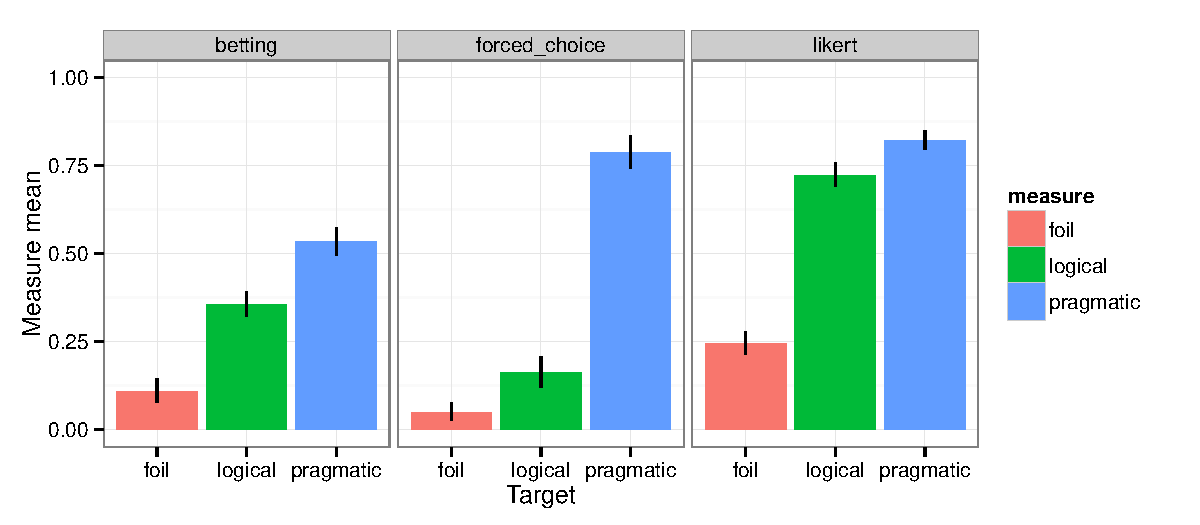
\includegraphics[width=6in]{../plots/1-prelims-dv.pdf}
  \caption{\label{fig:prelims-dv} Data from \exptref{exp:prelims-dv}. Each panel shows results from a different dependent variable (normalized for simplicity into the interval [0,1]). The three columns show results for the foil (e.g., $\emptyset$), logical (e.g., {\sc hg}), and pragmatic ({\sc g}) targets. Error bars show 95\% confidence intervals, computed by non-parametric bootstrap using the percentile method.}
\end{figure}

\exptref{exp:prelims-dv} explored the use of different dependent variables. We considered a betting measure, in which participants were instructed to allocate \$100 across the three targets, as in \citeA{frank2012}; a 7-point Likert scale, as in \citeA{goodman2013}; and a simple three-alternative forced choice measure.\footnote{As this experiment was one of our first and we were still actively developing items, we used only four of our six stimulus items: faces, boats, snowmen, and sundaes.} Figure \ref{fig:prelims-dv} shows results from each. With all three dependent variables, the pragmatic target was chosen more than the logical target, but this result was strongest for the forced choice, with 79\% of participants choosing the pragmatic target.

In contrast, both the Likert and betting measures afforded the possibility of ``hedging'' by allocating equal bets or ratings to the pragmatic and logical targets. Conservative participants took advantage of this possibility very frequently, betting equal amounts on the logical and pragmatic targets 43\% of the time and using equal Likert ratings 46\% of the time. The forced-choice dependent variable did not allow this kind of hedging; thus, we adopted it in our further experiments. In practice, these hedges might signal opportunities for clarification questions, a common response to ambiguity in more naturalistic communication \cite<e.g.,>{clark1989}.

\exptref{exp:prelims-mc} was designed to ensure that the presence of the manipulation check -- which asked participants to count how many of each feature was present -- did not induce a task demand that changed the magnitude of pragmatic responding. We saw 83\% pragmatic responding in the manipulation check condition and 77\% pragmatic responding in a matched condition with no manipulation check. Because of the high power of this experiment ($N_{include}$ = 513), the difference between conditions was statistically significant ($\chi^2(2) = 6.97,~p = .03$). Nevertheless, the modest (6\%) difference between conditions suggests that the manipulation check does not \emph{create} the pragmatic effect, though it may heighten participants' attentions to the different distributions of the two features, leading to slightly more pragmatic responding. We continue to use the manipulation check as an exclusion criterion in further experiments.

\exptref{exp:prelims-frame} was designed to test the particular linguistic framing we used. In particular, we contrasted the presentation of the target word (e.g., ``glasses'') as part of a phrase, ``Bob says: `My friend has glasses.'\,''\ and a presentation of the target word with the framing that the speaker can only say a single word (described above in the General Methods). The ``one word'' framing produced 80\% pragmatic responses, while the ``My friend has glasses'' framing produced 82\% pragmatic responses. These frames did not differ significantly from one another in the distribution of responses they produced ($\chi^2(2) = 2.54,~p = .28$). Except where noted below, we adopt the one-word framing.

In sum, these findings suggest that aspects of the experimental presentation and dependent variable have some minor effects on the magnitude of the pragmatic effect we observed. Nevertheless, the existence of the effect and its magnitude were quite robust to these variations.

\section{Measuring and manipulating prior expectations}
\label{sec:prior}

\exptrefrange{exp:prior-frame}{exp:prior-color} examine the role of prior expectations -- broadly construed -- in reference resolution through the kinds of reference games introduced above. These experiments serve two goals. First, they create a set of quantitative measurements of prior expectations combined with listener inferences; these measurements can be used for model comparison and assessment, a topic that we return to in the section on model fits below. Second, they allow causal inferences about the role of the prior in participants' pragmatic inferences. While \citeA{frank2012} \emph{measured} prior expectations and showed that they improved model fit, that work did not \emph{manipulate} prior expectations, so it was in principle possible that improvements in model fit did not result from a causal role played by prior expectations. We address this issue in the studies below. We begin by comparing methods for eliciting prior expectations (\exptref{exp:prior-frame}). We then investigate three ways of manipulating prior expectations: via base-rates (\exptref{exp:prior-baserate}), via linguistic valence (\exptref{exp:prior-valence}), and via perceptual salience (\exptref{exp:prior-color}).

It is not immediately clear what the best way is to measure prior expectations for purposes of communication. One particular conceptual issue seems important, though: does the term $P(r_S)$ refer to a prior over \emph{meaning}, that is, over speakers' particular communicative intentions? Or does it instead represent a prior over \emph{world states}, for example, the things the speaker would do, think about, or request? Although the distinction is subtle in most of our studies, the question of priors over meanings vs. states is a fairly deep philosophical issue.\footnote{See also \citeA{franke2009}, who notes that ``we should not conflate the [listener]'s possible conjectures about actualities with his preferred interpretations of expressions'' (p.129).}  In addition, if these two kinds of priors differ substantially, then our estimates of $P(r_S)$ might lead to incorrect conclusions.

\citeA{frank2012} introduced a method in which priors were measured identically to listener judgements, with the exception that participants in the prior measurement condition were not given any linguistic information. They were told that the speaker could utter one word to signal their target referent, but that they (the listener) hadn't heard it. This method yielded reliable measurements, but presupposed that the prior was over meanings, rather than world states.

\begin{figure}[t]
  \centering
  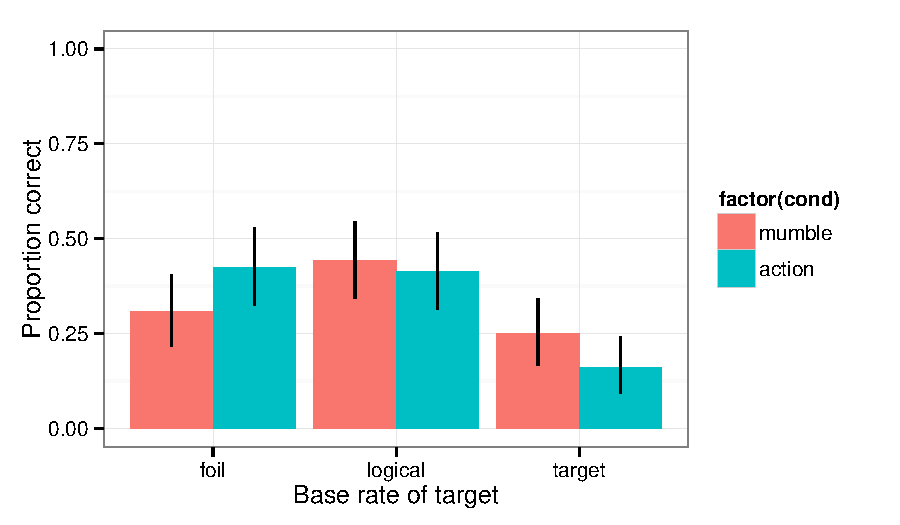
\includegraphics[width=5in]{../plots/2-prior-frame.pdf}
  \caption{\label{fig:prior-frame} Data from \exptref{exp:prior-frame}. Colors indicate different methods for eliciting prior expectations.}
\end{figure}

In \exptref{exp:prior-frame}, we compared prior elicitation methods. We presented participants with the same canonical display we had used in the earlier experiments, but asked them one of two prior questions. The meaning prior method was based on \citeA{frank2012}, where the participant was told that ``Bob can say one word'' but the word was presented as ``mumblemumble (you didn't hear what he said).'' The world state prior method consisted of simply asking, e.g., ``Which friend do you think Bob will visit next?'' A simple inferential test failed to show a significant difference in the distributions between the two questions ($\chi^2(2) = 3.45,~p = .18$, Figure \ref{fig:prior-frame}). While this failure is of course not decisive, in both conditions, participants showed a tendency to choose the logical target (e.g., face with both hat and glasses) most, the foil at intermediate rates, and the pragmatic target relatively less. This experiment does not resolve the underlying philosophical issue of what kinds of expectations the prior actually tracks. Given the limited empirical differences, however, we put aside this issue for the time being. Since the choice does not appear critical and the focus of our model is communicative behavior, we  adopt the meaning-based ``mumble" prior elicitation method for subsequent experiments.

\begin{figure}[t]
  \centering
  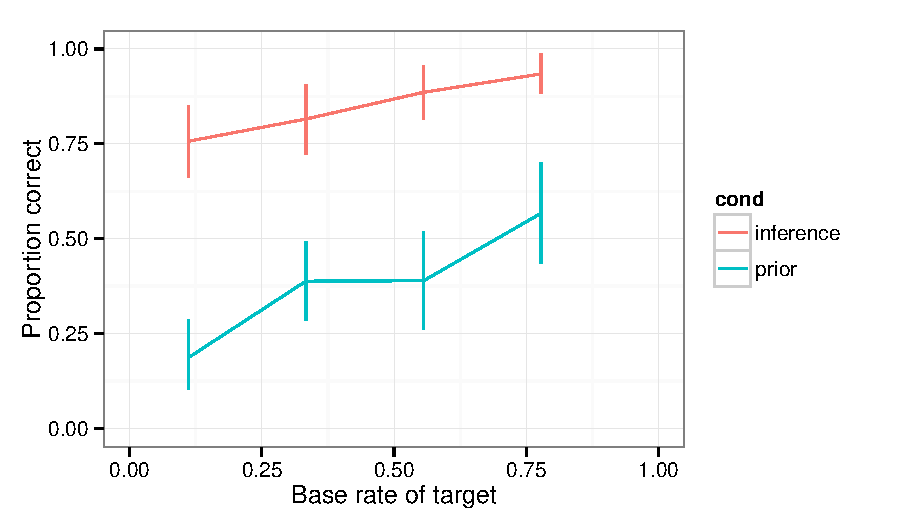
\includegraphics[width=5in]{../plots/2-prior-baserates.pdf}
  \caption{\label{fig:prior-baserate} Data from \exptref{exp:prior-baserate} from prior elicitation and inference conditions. Horizontal axis shows the proportion of familiarization trials that showed the pragmatic target.}
\end{figure}

In \exptref{exp:prior-baserate}, we attempted to manipulate participants' prior expectations about reference via a manipulation of the base rate of the interlocutor's actions.\footnote{This experiment is conceptually similar to a base-rate manipulation reported in \citeA{stiller2011}. However, the manipulation in that experiment used a different display, one more similar to those used in \exptref{exp:levels-level}.} The goal of this experiment was to provide evidence that prior expectations about actions influence inferences in the signaling games we were were studying -- licensing a causal inference about the role of priors.

Before to presenting the inference question in this experiment, we exposed participants to evidence about the habits of the interlocutor (Bob). The familiarization screen in this experiment stated (for example, in the case of the face stimulus) that Bob visited a friend every week; it then invited the participant to click on nine boxes to uncover the nine friends that Bob had visited most recently. Across four between-subjects base rate conditions, we manipulated how many of these boxes contained the pragmatic target (e.g., the face with glasses and no hat). One of the boxes always contained the foil (no glasses or hat) and another contained the logical target (hat and glasses). Then the other boxes contained either the pragmatic or the logical target. The four conditions were created such that 1/9, 3/9, 5/9, or 7/9 boxes showed the pragmatic target.

Figure \ref{fig:prior-baserate} shows the results of this manipulation.\footnote{This experiment had unusually high rates of exclusion due to participants' confusion about whether they should report familiarization frequencies for the manipulation check (instead of counts in the display). We maintain our strict inclusion criterion here but note that the results are largely unchanged if we include these participants.}  The base rate had a strong effect on the prior elicitation, but it also boosted levels of pragmatic inferences. To quantify these effects, we used a logistic regression model (no hierarchical model was warranted because judgments were from independent participants). This model showed highly significant effects of base rate ($\beta = .27,~p = .004$) and condition (with prior as the dummy-coded predictor, $\beta = -.57,~p < .0001$), as well as a marginal interaction of the two  ($\beta = .29,~p = .06$). Critically, the main effect of base rate remained reliable in a similar logistic regression for just the inference trials ($\beta = .28,~p = .0001$), indicating a highly reliable (and graded) effect of the base-rate manipulation on the strength of the pragmatic inference.


\begin{figure}[t]
  \centering
  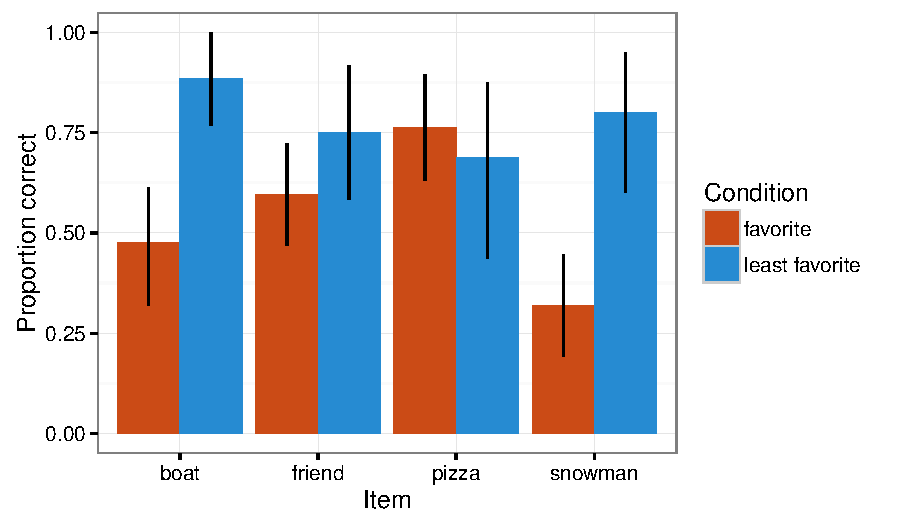
\includegraphics[width=6in]{../plots/2-prior-valence-items.pdf}
  \caption{\label{fig:prior-valence} Data from \exptref{exp:prior-valence} from the inference conditions, broken down by item.}
\end{figure}

Our next experiment, \exptref{exp:prior-valence}, investigated the effects of linguistic manipulations on participants' priors and their resulting inferences. The goal of this experiment was to test whether, like base rate information, other, more subtle, manipulations of prior expectations would be integrated into the (putatively pragmatic) judgments we observed. In this experiment, we framed judgments as being about determining Bob's \emph{favorite} or \emph{least favorite} item. This experiment was conducted chronologically earlier in the sequence and had four rather than six experimental items: faces, boats, pizzas, and snowmen.

In the prior condition, the data overall supported the conclusion that Bob's favorite item would likely have more features, while his least favorite would likely have fewer. The logical option, which had the most features, was chosen as ``favorite'' 70\% of the time, while the distractor option, which had zero features, was chosen as ``least favorite'' 77\% of the time.

In the inference condition, however, the linguistic manipulation had different results across items, as seen in Figure \ref{fig:prior-valence}. Put simply, if your least favorite boat has a sail, it's likely to have no other features; in contrast, if your favorite boat has a sail, it's likely to have other features as well. The same was true of snowmen as well. But for pizzas, if your favorite \emph{or} your least favorite has mushrooms, it is likely to have little else on it. Presumably participants reasoned that, if you like mushrooms, you want lots of them, and if you don't like them, you would be most upset if they were alone, unmasked by any other topping. Confirming this impression of the data, a logistic regression predicting target responses as a function of item and condition showed a significant interaction between linguistic condition and the (dummy coded) pizza item ($\beta = -2.51$, $p = .008$). Thus, this experiment demonstrates that participants' prior expectations about the importance of particular features for a particular domain interacted with their willingness to make a pragmatic implicature.

\begin{figure}[t]
  \centering
  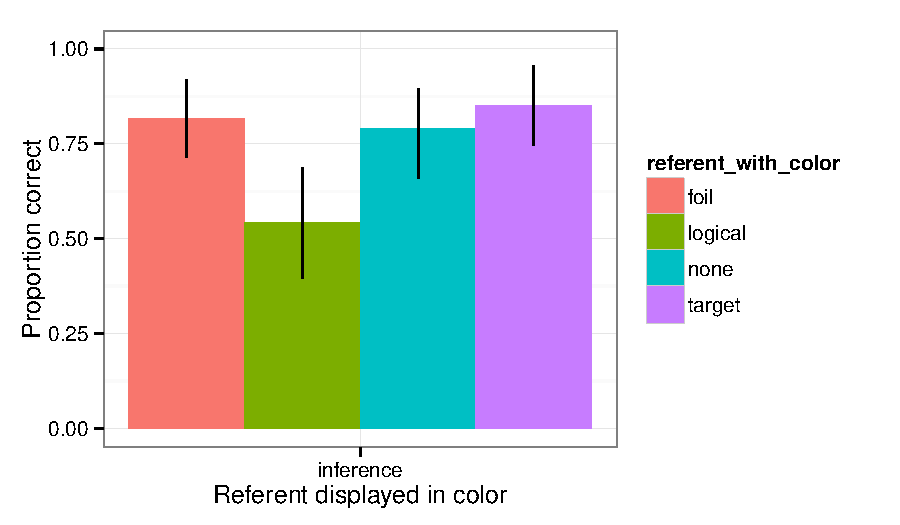
\includegraphics[width=4in]{../plots/2-prior-color.pdf}
  \caption{\label{fig:prior-color} Data from \exptref{exp:prior-color} in the inference conditions.}
\end{figure}

Our final experiment in this sequence, \exptref{exp:prior-color}, attempted to manipulate prior expectations about reference by changing the salience of the different referents. The goal of this experiment was to use a more obvious, perceptual manipulation of expectations (compared with \exptref{exp:prior-valence}). In particular, we presented all but one of the images in grayscale, varying which of the images (pragmatic target, logical target, or foil) was shown in color.\footnote{To ensure that participants still made the inference more generally, we included a condition where none of the referents was shown in color, notated by ``none.''} This manipulation had a strong effect on pragmatic inferences. In particular, when the logical target was shown in color, inferences to the pragmatic target dropped significantly (Figure \ref{fig:prior-color}; in a logistic regression, $\beta = -1.42$, $p = .003$), presumably because the color either drew attention to the logical target or signaled to participants that their attention \emph{should be} drawn to the logical target.

In sum, \exptrefrange{exp:prior-baserate}{exp:prior-color} together show strong evidence that many information sources can affect prior expectations about reference. In particular, these experiments license two inferences. First, manipulations that affect prior expectations about what a speaker will talk about (and, potentially, do) have a causal effect on inferences in signaling games. Second, these manipulations were reflected in the global rate of inference in a graded fashion that appeared quite sensitive to their type and magnitude. We return to these data below and use the RSA model to test the hypothesis that variation in inference levels can be accounted for by variation in prior expectations.

\section{Levels of recursion and limits on human reasoning}
\label{sec:levels}

\exptrefrange{exp:levels-level}{exp:levels-oddman} probe the limits on the kind of inferences participants can make in our reference game paradigm. The general goal of these experiments was to test whether the inference we saw so robustly above in the ``simple'' signaling game would generalize to others with more varied arrangements of features. In all of these experiments, we also conducted parallel experiments measuring prior expectations using the methods described above, but we largely omit discussion of these data until we use them for model fitting below.

 \begin{figure}[t]
  \centering
  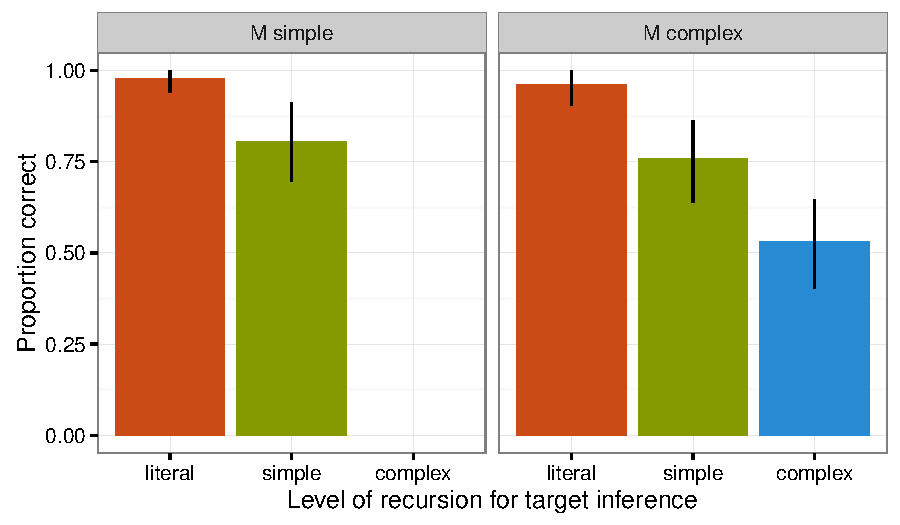
\includegraphics[width=5in]{../plots/3-levels-levels.pdf}\\
  \hspace{6ex} 
\includegraphics[width=2in]{figures/hatglasses.pdf}\hspace{2ex}
  
\includegraphics[width=2in]{figures/levels-levels-stim.pdf}
  \caption{\label{fig:levels-level} Data from \exptref{exp:levels-level}, plotted by display (left: simple, right: complex) and inference level (see text).}
\end{figure}

In our first experiment, \exptref{exp:levels-level}, we measured patterns of inference in more complex reference games. Following \citeA{stiller2011} and \citeA{degen2012}, we created a signaling game that required a somewhat deeper level of reasoning than our previous experiments. In particular, we compared our standard reference game (shown again for reference in Figure \ref{fig:levels-level}, bottom left) alongside a more complex game (Figure \ref{fig:levels-level}, bottom right):

\begin{equation}
    M_{complex} = \kbordermatrix{
      & \textsc{m} & \textsc{gm} & \textsc{hg} \\
      hat & 0 & 0 & 1  \\
      glasses & 0 & 1 & 1 \\
      mustache & 1 & 1 & 0 \\
    }
\end{equation}

Different reference games require different depths of recursion to achieve a solution. We define a solution for a listener as a state where each message can be mapped to a particular referent (e.g., has a unique maximum value), and for a speaker as a state where each referent has a corresponding message (similarly, has a unique max). (Of course, some matrices do not have such solutions at all, but if a matrix is solved for a speaker, it is solved for all deeper listeners and vice versa.) For example, the ``simple'' matrix, which we have studied in the previous experiments, reaches a solution state with only half a level of recursion: As shown in the worked example above, a model that implements $S(L(M_{simple}))$ will show an implicature. In contrast, in the ``complex" matrix, $L(S(L(M_{complex})))$ is required for one of the potential implicatures (that ``glasses'' refers to {\sc gm}).

In \exptref{exp:levels-level}, we used the stimulus in Figure \ref{fig:levels-level}A to measure inferences about the previous pragmatic target (``glasses" interpreted as {\sc g}, as in $M_{simple}$) and the target with the unique feature (``hat" means {\sc hg}). We also used the stimulus in Figure \ref{fig:levels-level}B to measure the more complex pragmatic inference (the target for this inference was {\sc m} for ``mustache''). The main contribution of this experiment, however, was our test of the $L(S(L(M)))$ inference (``glasses'' implicating {\sc gm}). This inference depends on having reasoned that, while both of the targets have another possible descriptor, for one of those targets, the second descriptor is unique, whereas for the other the second descriptor is also non-unique. As the preceding description shows, such reasoning is non-trivial.

Figure \ref{fig:levels-level} shows the findings. Judgments in the simpler inference remained very close to 75\% (the level observed across many of our other experiments), regardless of display. Literal meaning judgments were at ceiling. In contrast, more complex inferences were at chance (53\%). The prior for this target was lower than the prior for the logical distractor image, however (23\% vs 39\%). Thus, it may be the case that participants make this inference but it was partially or fully cancelled  by an expectation against it (see Figure 1 of Frank \& Goodman, 2012, for a potential example of this kind of cancellation, and see the next section for further discussion).

 \begin{figure}[t]
  \centering
  \includegraphics[width=4in]{../plots/depth2.pdf}
  \caption{\label{fig:really-hard} An example signaling game for which a solution is present for $L_2$ but not $L_1$.}
\end{figure}

We considered conducting experiments with more complex signaling games that required deeper levels of recursion to achieve a solution for some messages. Brute-force searches of the space of possible matrices returns examples like Figure \ref{fig:really-hard}, with

\begin{equation}
    M = \kbordermatrix{
      & \textsc{gm} & \textsc{hg} & \textsc{h} & \textsc{gm} \\
      hat      & 0 & 0 & 1 & 1  \\
      glasses  & 0 & 1 & 1 & 1 \\
      mustache & 1 & 1 & 0 & 0 \\
    }
\end{equation}

and

\begin{equation}
    L(S(L(S(L(M))))) = \kbordermatrix{
      & \textsc{gm} & \textsc{hg} & \textsc{h} & \textsc{gm} \\
hat      & 0.00 & 0.00 & 0.50 & 0.50 \\
glasses  & 0.00 & 0.37 & 0.31 & 0.31 \\
mustache & 0.50 & 0.50 & 0.00 & 0.00 \\
    }.
\end{equation}

The key result for this matrix is that, at $L_2$ but not $L_1$, ``glasses'' implicates {\sc hg}. But the numerical difference is quite tiny (leading us to question whether we could measure such an effect), and the intuition felt even weaker than in the ``complex'' game (of which this matrix is a variant). Thus, we chose not to run these experiments.

 \begin{figure}[t]
  \centering
  
\includegraphics[width=3in]{figures/levels-twins-stim.pdf}
  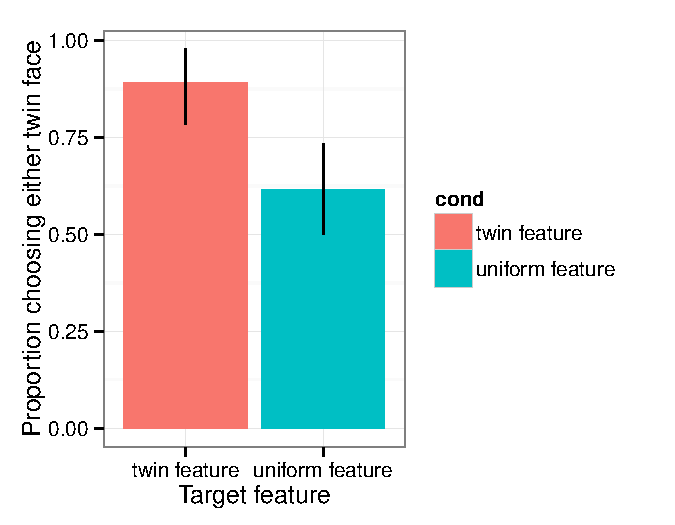
\includegraphics[width=3in]{../plots/3-levels-twins.pdf}
  \caption{\label{fig:levels-twins} Data from \exptref{exp:levels-twins}, along with the display used for this experiment.}
\end{figure}

\exptrefrange{exp:levels-twins}{exp:levels-oddman} further considered the scope of the inferences that participants make. In particular, these experiments had as a goal asking whether participants would ever violate the literal semantics of the messages (especially in cases where it would otherwise be impossible to refer to a particular object). We began by examining displays like the one shown in Figure \ref{fig:levels-twins}, top:

\begin{equation}
    M = \kbordermatrix{
               & \textsc{gm} & \textsc{hm} & \textsc{hm} \\
      hat      & 0  & 1  & 1  \\
      glasses  & 1  & 0  & 0 \\
      mustache & 1  & 1  & 1 \\
    }
\end{equation}

\noindent These displays had a uniform feature and another feature that was shared by two of the three objects. Intuitively, naming the unique feature (``glasses'') should reference the object with it ({\sc gm}). But the predictions for the other features were perhaps less clear. Should the uniform feature also resolve to the unique object (e.g., ``mustache'' means {\sc gm})? And should ``hat'' resolve ambiguously to the duplicated objects ({\sc hm}), or to the non-duplicated object ({\gm}), violating the literal semantics of the message?

Referencing the duplicated feature (``hat'') led most participants to choose one of the duplicated referents ({\sc hg}), suggesting that they did not violate the literal semantics (Figure \ref{fig:levels-twins}). The message that applied to all three objects (``mustache") led to a standard implicature (as in the ``simple'' matrix). Like \exptref{exp:levels-level}, this experiment provided some evidence for the robustness of the basic implicature phenomenon.

 \begin{figure}[t]
  \centering
  
\includegraphics[width=3in]{figures/levels-oddman-stim.pdf}
  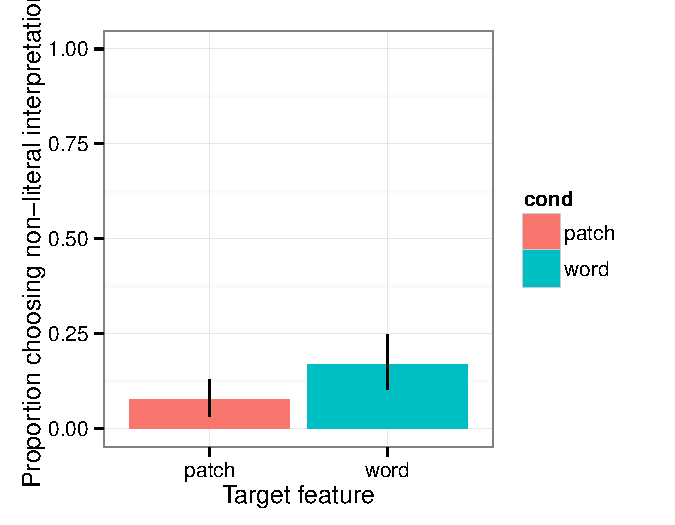
\includegraphics[width=3in]{../plots/3-levels-oddman.pdf}

  \caption{\label{fig:levels-oddman} Data from \exptref{exp:levels-oddman}, along with the display used for this experiment.}
\end{figure}

\exptref{exp:levels-oddman} further considered whether participants would reach communicative equilibria that were at odds with those implied by the literal semantics of the words the speaker used, in cases where the matrix was systematically and frustratingly ambiguous. To address this question, we used a display like the one in Figure \ref{fig:levels-oddman}, top:

\begin{equation}
    M = \kbordermatrix{
               & \textsc{hg} & \textsc{hm} & \textsc{gm} \\
      hat      & 1  & 1  & 0  \\
      glasses  & 1  & 0  & 1 \\
      mustache & 0  & 1  & 1 \\
    }
\end{equation}

\noindent Although every feature was ambiguous, a potential equilibrium would be the use of a particular feature to describe the target \emph{without} that feature. For example, here ``hat'' could refer to the face without a hat; ``glasses'' to the face without glasses; etc. But by and large, participants did not converge on this equilibrium and instead were content to choose between the two ambiguous referents (\ref{fig:levels-oddman}, bottom, word condition), with only 17\% of participants choosing to violate the literal semantics.

A second condition examined whether participants would be more or less likely to abandon the signal if it were an unconventional signal rather than a word with conventional semantics. In this condition, we recolored the features of each object (e.g., the hat and glasses) so that each had its own unique color. Bob then communicated by showing a color patch corresponding to the matching feature. Contra our initial prediction, participants stuck \emph{more} closely to the match between color patches and particular features, choosing the ``odd man out'' at very low rates (8\%). This condition suggests that it may be a feature of reasoning in these signaling games (rather than of words per se) that keeps participants from abandoning the literal semantics of the particular signals the communicator uses.

These results contrast with recent findings from \citeA{misyak2016}, who studied whether a particular signal's meaning could reverse in a signaling game where participants communicated about hidden objects. They found that signals could be used flexibly to indicate the locations of either rewards or dangers, depending on the particular constraints and affordances of the communicative situation. Messages in their study were ``tokens" that were placed on top of locations in a virtual world, however, perhaps suggesting a more flexible semantics (e.g., ``something [good or bad] is in here'') than the words and color patches we used in our studies. In addition, though they saw conventions appear even without repeated communication with a single partner, all participants in their studies built up some practice with the constraints of the virtual world of the game. In contrast, our participants got only a single opportunity to reason about a wholly-new set of constraints. More work will be needed to determine what aspects of the communicative task allow or prevent the emergence of reversible semantic conventions.

In sum, these experiments suggest the basic pragmatic inferences of the type studied throughout this paper were robust across a variety of displays (for example in the new matrix types shown in \exptrefrange{exp:levels-level}{exp:levels-twins}). But we saw very little evidence that, in a one-shot game of the sort studied here, participants would  abandon the literal semantics of the words that were used \cite<cf.>{misyak2016}. And the evidence for inferences at deeper levels of recursion was limited at best \cite<cf.>{franke2016}. Whether these are limitations of our paradigm or of human pragmatic reasoning more generally will require further study.

\section{Model fits and model comparison}
\label{sec:modelcomp}

In the experiments reported above, we saw strong evidence that participants are engaging in reasoning that goes beyond the simple semantic interpretation of messages. Instead, they appear to be making inferences about reference in context that have the character of pragmatic reasoning -- considering inferential alternatives that a speaker could have said. In this section, we test the ability of the RSA model to describe human behavior in these experiments.


\subsection{Model comparison methods}

For each experiment in the second and third sequences (\exptrefrange{exp:prior-baserate}{exp:levels-oddman}), we compared predictions of the RSA model to participant data. As in \citeA{frank2012}, for each experiment and experimental condition, we compared the proportion of participants choosing each different target to the model's predictions about that target (e.g., proportion choosing target {\sc h}, {\sc hg}, etc.). This procedure yielded between 4 and 10 datapoints per experiment.

We used an implementation of the RSA model provided by a new package for the R statistical computing platform: \texttt{rrrsa}. The package is available at \url{http://github.com/benpeloquin7/rrrsa} and installation instructions and comprehensive documentation are also available at that link.\footnote{The \texttt{rrrsa} package is optimized for analysis of experimental data like those presented here; other, more flexible variants of RSA models are available for exploration and extension at \url{http://forestdb.org/models/scalar-implicature.html} and \url{https://github.com/cgpotts/pypragmods}.}

When we propagate empirical prior information into the model, we compute confidence intervals by simulating model fit using a non-parametric bootstrap resampling procedure in which the prior data are resampled with replacement and then the model is rerun 500 times using these resampled priors. Error bars then reflect percentile-based confidence intervals computed from these simulations.

Throughout, we assess model fit to data using a simple Pearson correlation statistic. Although a good fit alone cannot be probative \cite{roberts2000}, the RSA model as stated here and earlier contains a small number of parameters: depth of recursion and $\alpha$ (the greed parameter in the choice rule). We believe the use of correlations is relatively unproblematic since (as we show) changes in these parameters do not result in any radically different patterns of model predictions. Nevertheless, we do caution that our comparisons between models are exploratory (rather than being fully-preplanned confirmatory tests) and serve to elucidate differences in fit, rather than being a formal basis for quantitative model comparison. In particular, even if there are differences in fit between models, such a result doesn't guarantee better performance across stimulus conditions or parameters other than those evaluated here.

\subsection{RSA models achieve globally good fit to experimental data}

\begin{figure}[t]
 \centering
 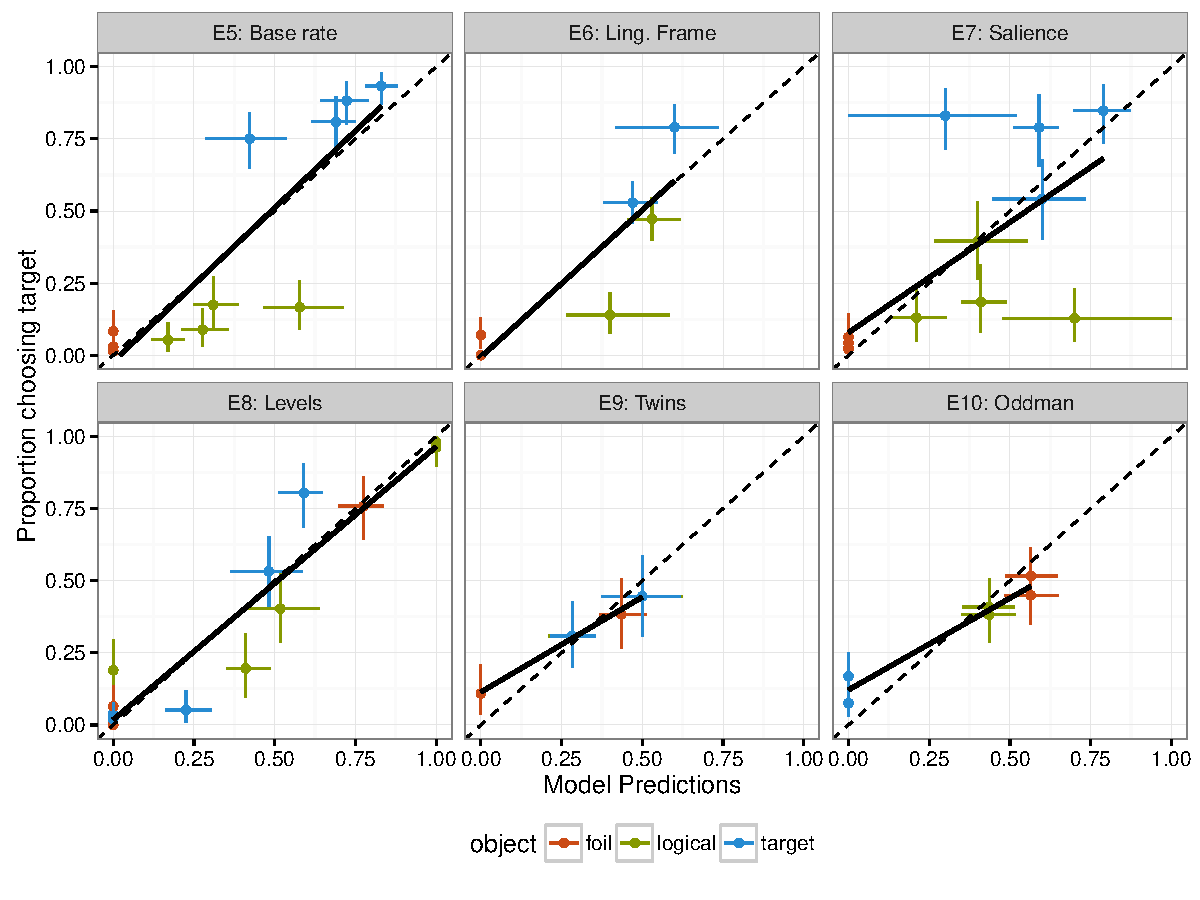
\includegraphics[width=6in]{../plots/model_basic.pdf}
 \caption{\label{fig:basic} Human data plotted against RSA model predictions for a recursive depth of 1, and $\alpha=1$. Each point shows proportion of choices for a single target object. Colors denote the pragmatic target (e.g., glasses), logically true object (e.g., hat and glasses), foil (e.g., no hat, no glasses). Vertical error bars are binomial confidence intervals; horizontal error bars are computed by resampling prior data and recomputing model predictions (see text). Black lines show the line of best fit.}
\end{figure}

In our first simulation, we used the exact version of the RSA model given in \citeA{frank2012}, with a recursive depth of 1 and $\alpha=1$. Results of this simulation are given in Figure \ref{fig:basic}. The RSA model was correlated with human judgments ($r_{all} = .86$), and this correlation persisted even when removing those points predicted to be 0 or 1 ($r_{no~0/1} = .68$).\footnote{For \exptref{exp:prior-color} -- and to a lesser extent, for \exptref{exp:prior-valence} -- we saw a number of conditions in which model predictions had very high variance. This variance arises from variability in the prior on particular objects (since they are chosen very infrequently in the prior condition, they show high numerical instability).}

Nevertheless, there were a number of experimental conditions for which this parameter setting did not yield good predictions. In \exptrefrange{exp:prior-baserate}{exp:levels-level}, there appears to be a trend in which the model overpredicts for options that are judged to be lower probability, and underpredicts for those options judged more likely by participants. (This trend manifests itself as a cluster of predictions that are too close to the vertical midline of $p_{model}=.5$). In order to explore this trend further, we next varied the recursive depth in the model. Intuitively, further recursion should strengthen pragmatic inferences.

\subsection{Deeper recursion improves model performance}

% latex table generated in R 3.3.0 by xtable 1.8-2 package
% Wed Jul  6 10:15:12 2016
\begin{table}[ht]
\centering
\begin{tabular}{rrr}
  \hline
Depth & $r_{all}$ & $r_{no~0/1}$ \\
  \hline
  0 & 0.74 & 0.14 \\
    1 & 0.86 & 0.68 \\
    2 & 0.93 & 0.86 \\
    3 & 0.95 & 0.90 \\
    4 & 0.95 & 0.91 \\
    5 & 0.95 & 0.91 \\
   \hline
\end{tabular}
\caption{\label{tab:corr-a1} Correlations of model and data on both the full dataset and the subset of conditions for which the model did not predict a probability of either 0 or 1.}
\end{table}

Table \ref{tab:corr-a1} shows the results of simulations at depths 0 - 5. These results show two main findings. First, and critically, a single level of recursion dramatically improves performance over and above a flat (literal listener) model. This trend is especially pronounced for non-binary model predictions. Indeed, our experiments were designed to probe cases where a literal listener would make equal predictions for different objects but a pragmatic agent would differentiate between them. Thus, this result provides a (perhaps obvious, but still important) confirmation of our basic hypothesis, namely, that participants reason pragmatically in our experiments.

\begin{figure}[t]
 \centering
 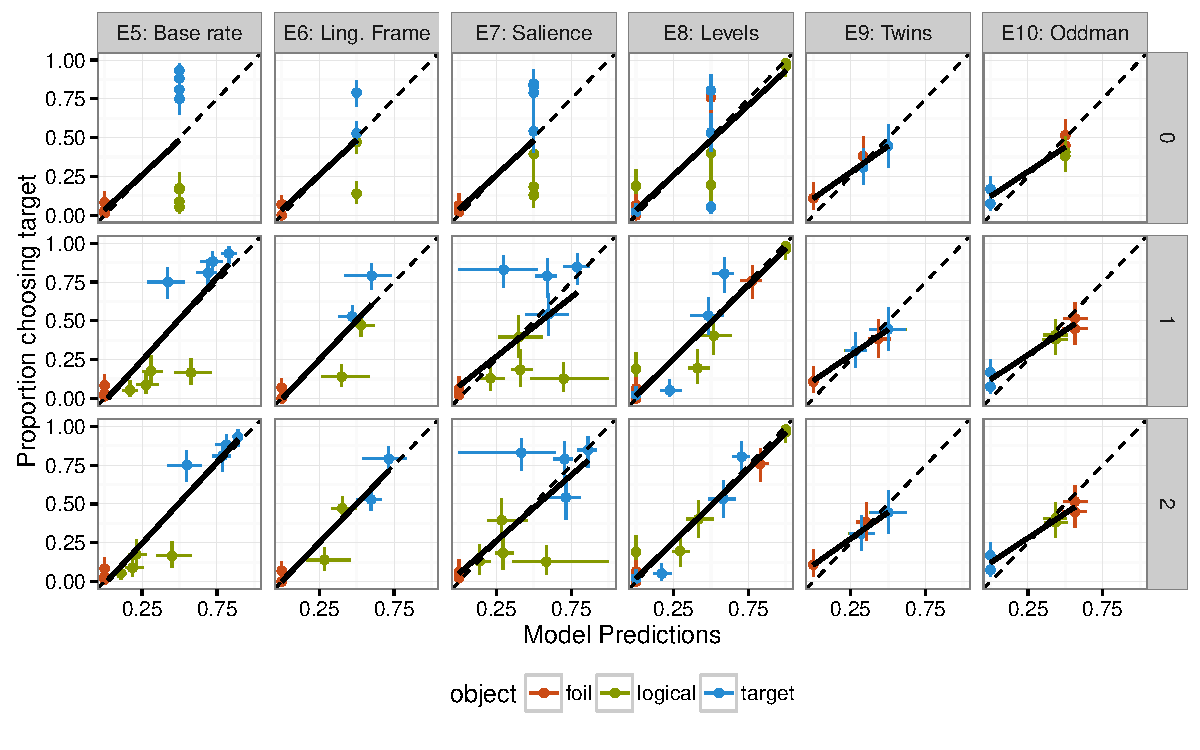
\includegraphics[width=6in]{../plots/model_depth.pdf}
 \caption{\label{fig:depths} Human data plotted against RSA model predictions for recursive depths 0 -- 2 (shown as different rows of panels), and $\alpha=1$. Plotting conventions are as above.}
\end{figure}

Second, however, the simulations showed an unexpected finding: deeper levels of recursion correlated more highly with human judgments. In particular, even four levels of recursion improved fit numerically compared with three levels (especially for non-0/1 predicted values). Figure \ref{fig:depths} shows simulation results at depths 0 -- 2 (the middle row is identical to Figure \ref{fig:basic}); we do not plot depths 3 -- 5 because they are visually almost indistinguishable from depth 2 even though there are minor numerical differences in their correlation with participant data.

Recall, however, that we set the $\alpha$ parameter to 1 in these simulations. $\alpha$ controls the ``greediness'' of the model's choice rule, with higher values indicating a greater willingness to choose higher-probability options. In the next set of simulations, we let $\alpha$ vary.

\subsection{The $\alpha$ parameter trades off with recursive depth, limiting model-depth identifiability}

\begin{figure}[t]
 \centering
 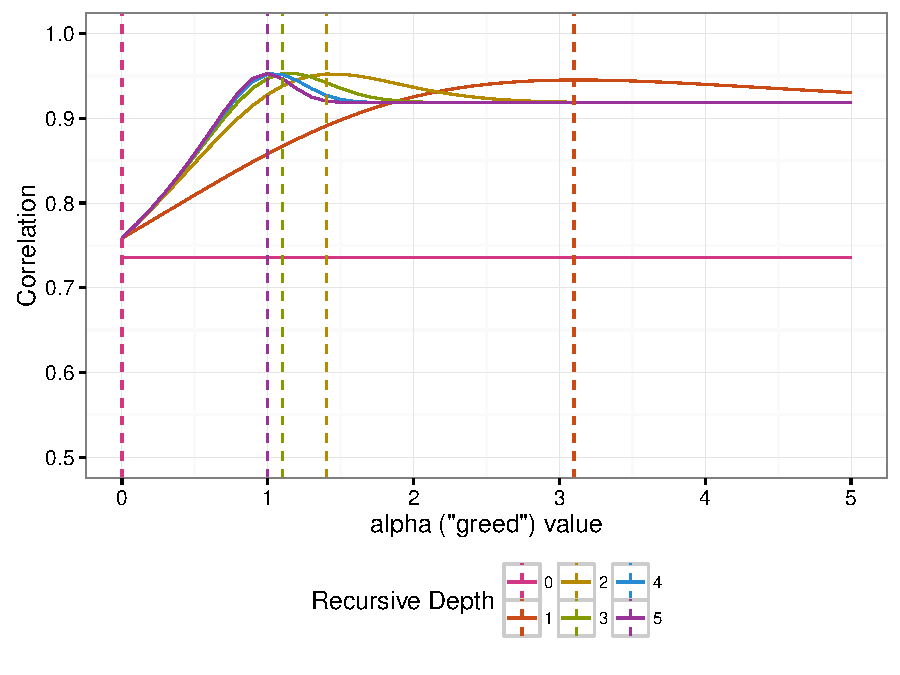
\includegraphics[width=5in]{../plots/alpha-fit.pdf}
 \caption{\label{fig:alpha-fit} Correlation between full human dataset and RSA models at different levels of $\alpha$. Colors show levels of recursive depth from 0--5, dashed lines mark the maximum correlation for each depth.}
\end{figure}

% latex table generated in R 3.3.0 by xtable 1.8-2 package
% Thu Jul  7 09:53:32 2016
\begin{table}[ht]
\centering
\begin{tabular}{rrrr}
  \hline
Depth & $\alpha_{best}$ & $r_{all}$ & $r_{no~0/1}$ \\
  \hline
  0 & 0.0 & 0.74 & 0.14 \\
    1 & 3.1 & 0.95 & 0.89 \\
    2 & 1.4 & 0.95 & 0.91 \\
    3 & 1.1 & 0.95 & 0.91 \\
    4 & 1.0 & 0.95 & 0.91 \\
    5 & 1.0 & 0.95 & 0.91 \\
   \hline
\end{tabular}
\caption{\label{tab:corrs-fita} Correlations of model and data (as above) with best-fitting $\alpha$ value at each depth.}
\end{table}

Figure \ref{fig:alpha-fit} shows the range of correlations with human data achieved at different levels of $\alpha$, across recursive depths; Table \ref{tab:corrs-fita} gives the highest correlation and corresponding $\alpha$ level. Two findings become apparent. First, at the highest level, although numerical correlations do vary across $\alpha$ levels, with $\alpha > 1$ the range of correlations is quite restricted across all depths. Thus, the performance of the model is relatively insensitive to this parameter.

Nevertheless, a close examination of Table \ref{tab:corrs-fita} shows that values at depth 2 and especially depth 1 are noticeably higher than in Table \ref{tab:corr-a1} where $\alpha=1$. In fact, by setting $\alpha=3.1$, a model with depth 1 still achieves just about the same level of fit to data as a model with depth 4 or 5. This finding suggests that $\alpha$ and depth trade off against one another in most of the experiments that we conducted.

To understand this result, consider the standard matrix we used in most of our experiments (reproduced from above):

\begin{equation}
      M = \kbordermatrix{
                 & \emptyset & \textsc{g} & \textsc{hg} \\
        hat      & 0  & 0  & 1  \\
        glasses  & 0  & 1  & 1 \\
      }
\end{equation}

\noindent In this case, recursive depth 1 and $\alpha=1$ produces:

\begin{equation}
      L(S(L(M))) = \kbordermatrix{
                 & \emptyset & \textsc{g} & \textsc{hg} \\
        hat      & 0  & 0  & 1  \\
        glasses  & 0  & .75  & .25 \\
      }
\end{equation}



\noindent But note that recursive depth 2 produces:

\begin{equation}
  L(S(L(S(L(M))))) = \kbordermatrix{
             & \emptyset & \textsc{g} & \textsc{hg} \\
    hat      & 0  & 0  & 1  \\
    glasses  & 0  & .83  & .17 \\
  }
\end{equation}

\noindent which is identical to the same result at recursive depth 1 with $\alpha = 2$. But that is not always true. In principle, if a particular matrix is completely ambiguous at a particular recursive depth, then changing $\alpha$ will not affect performance. For example, the symmetry for the two identical elements in the matrix in \exptref{exp:levels-twins} cannot be broken by changing $\alpha$. (Another, more trivial, example of this observation would be changing levels of $\alpha$ for a literal listener; clearly this manipulation would have no effect since by definition the literal listener assigns probability evenly to all alternatives.)

\subsection{Priors do not improve global fit and also trade off with $\alpha$ and recursive depth}

\begin{figure}[t]
 \centering
 \includegraphics[width=6in]{../plots/model_noprior_depth.pdf}
 \caption{\label{fig:noprior} Human data plotted against RSA model predictions for recursive depths 0 -- 2, and $\alpha=1$. RSA model does not include estimates of the prior, hence there are no error bars on the horizontal axis. Plotting conventions are as above.}
\end{figure}

% latex table generated in R 3.3.0 by xtable 1.8-2 package
% Thu Jul  7 11:16:06 2016
\begin{table}[ht]
\centering
\begin{tabular}{rrr}
  \hline
  Depth & $r_{all}$ & $r_{no~0/1}$ \\
  \hline
  0 & 0.74 & 0.14 \\
    1 & 0.94 & 0.90 \\
    2 & 0.95 & 0.90 \\
    3 & 0.95 & 0.90 \\
    4 & 0.94 & 0.90 \\
    5 & 0.94 & 0.90 \\
   \hline
\end{tabular}
\caption{\label{tab:corrs-noprior} Correlations of no-prior model and data at varying recursive depths.}
\end{table}

The final issue we examine is the contribution of empirically-determined priors to overall model fit. We began with a model that used empirical prior measurements because \citeA{frank2012} proposed that they were necessary. Despite this previous work, we found that global fit of a model with $\alpha=1$ and no prior was equivalent to the performance of the fitted-$\alpha$ model \emph{with} priors. Correlations are shown in Table \ref{tab:corrs-noprior}; numerically, results are almost identical with those shown in Table \ref{tab:corrs-fita}. Levels of recursion from 0--2 are shown visually in Figure \ref{fig:noprior}.\footnote{We also experimented with incorporating the prior at every level of recursion, rather than only at the top level of recursion. This model variant corresponds to a scenario in which the prior is mutually-known to both communicators (and they reason pragmatically about that mutual knowledge). In contrast the case we presented above corresponds to a scenario where the prior represents information that only the listener has access to (e.g., about perceptual salience or personal expectations about the situation). We found that the ``mutual knowledge'' variant performed worse than either the no-prior or the ``private knowledge'' model (the one presented in the main text) in all cases, with the fitted-$\alpha$ correlations lower by .02-.05 depending on the level of recursion.}

It is surprising that the use of the empirical prior fails to improve model fit. Yet despite this lack of global improvement, we note that there is unambiguous evidence from \exptrefrange{exp:prior-baserate}{exp:prior-color} that manipulations of participant expectations about the target object lead to altered pragmatic judgments. In \exptref{exp:prior-baserate} in particular, we saw that manipulations of the base rate of a target object led to quantitative changes in both prior measurements and rates of pragmatic inference.

% latex table generated in R 3.3.0 by xtable 1.8-2 package
% Thu Jul  7 11:39:37 2016
\begin{table}[ht]
\centering
\begin{tabular}{clrrrrrr}
  \hline
Depth & Model & E5 & E6 & E7 & E8 & E9 & E10 \\
  \hline
  1 & No prior, $\alpha=1$ & 0.96 & 0.89 & {\bf 0.95} & 0.96 & 0.88 & 0.95 \\
    1 & Prior, $\alpha$ fit & {\bf 0.99} & {\bf 0.93} & 0.89 & {\bf 0.97} & 0.75 & {\bf 0.98} \\
    1 & Prior, $\alpha=1$ & 0.87 & 0.87 & 0.67 & 0.95 & {\bf 1.00} & {\bf 0.98} \\
  \hline
    2 & No prior, $\alpha=1$ & {\bf 0.99} & 0.87 & {\bf 0.95} & 0.97 & 0.80 & 0.95 \\
    2 & Prior, $\alpha$ fit & {\bf 0.99} & 0.93 & 0.89 & {\bf 0.98} & 0.84 & {\bf 0.98} \\
    2 & Prior, $\alpha=1$ & 0.95 & {\bf 0.96} & 0.81 & {\bf 0.98} & {\bf 0.99} & {\bf 0.98} \\
  \hline
    3 & No prior, $\alpha=1$ & {\bf 0.99} & 0.86 & {\bf 0.95} & 0.97 & 0.74 & 0.95 \\
    3 & Prior, $\alpha$ fit & {\bf 0.99} & 0.93 & 0.89 & {\bf 0.98} & 0.89 & {\bf 0.98} \\
    3 & Prior, $\alpha=1$ & 0.98 & {\bf 0.95} & 0.86 & {\bf 0.98} & {\bf 0.95} & {\bf 0.98} \\
  \hline
\end{tabular}
\caption{\label{tab:expts-corrs} Correlations of model and data for three model variants and varying recursive depths, broken down by experiment. Results for depths 4 and 5 are similar to depth 3. $\alpha$ values are fit globally rather than individually for each experiment.}
\end{table}

We discuss two observations about this unexpected finding: that there are tradeoffs between the prior, $\alpha$, and depth of recursion and that there may be measurement issues that complicate model comparisons. These observations are based on an analysis of the individual correlations, separated by experiment (Table \ref{tab:expts-corrs}).

First, intuitively and as illustrated above, both increases in $\alpha$ and increases in recursive depth function to ``pull apart'' different targets, increasing the highest probability option and decreasing the lowest probability option. A comparison of Figures \ref{fig:depths} and \ref{fig:noprior} suggests that including empirical prior measurements tends to exert the opposite pressure. In fact, this observation reveals an interesting generalization about our displays: our pragmatic targets tend to be \emph{less} salient than our logical targets. For example, in the canonical display we use, the face with a hat is less salient than the display with the hat and glasses. Including information of this sort about salience via the empirical prior then works \emph{against} the pragmatic inference, even as both increasing $\alpha$ and recursive depth strengthen the inference. Another way to think about this observation is that, in cases that the pragmatic target is more salient, it will reliably be picked by $L_0$ -- such cases may not even appear pragmatic since no reasoning is necessary.

Second, adding empirical priors to the model complicates quantitative comparison with no-prior models substantially. Although adding the empirically-measured prior does not add any free variables to the model, it does add substantial measurement-related noise (consider the error bars shown in Figure \ref{fig:depths} but not Figure \ref{fig:noprior}). Thus, a failure to see increases in overall fit to data may be the result of a tradeoff between better fit in some cases due to the prior better accounting for the structure of the data \emph{and} worse fit due to the prior measurements introducing random noise. In addition, errors due to random noise are systematic: They bias extreme values towards the center. This systematic bias would almost certainly reduce global fit to data, although quantifying its magnitude might be difficult.

\section{General Discussion}
\label{sec:discussion}

The flexibility of comprehension in context is one of the most important and striking features of human language. Yet in contrast to theories of syntax and semantics \cite<e.g.,>{chomsky1965,jackendoff2002}, the most influential pragmatic theories have typically been quite informal in nature \cite{grice1975,sperber1986,clark1996,levinson2000}. This gap has been addressed by recent efforts to develop probabilistic models of pragmatic reasoning, inspired by developments in game theory \cite<e.g.,>{benz2005} and social cognition \cite{baker2009}.

In the current work, we gave an extended presentation of one particular class of probabilistic pragmatics model: the rational speech act, or RSA, model \cite{frank2012,goodman2013}. Although a variety of models in this family have been presented previously, we provided a more extended description and comparison to other related models (along with software for using basic RSA models for simulations). We then conducted a series of large-scale, single-judgment pragmatic inference experiments to validate and explore one-shot reference games as a method for studying pragmatic inference quantitatively.

These experiments support three main conclusions. First, language games of the type we studied here are a flexible and robust tool for probing pragmatic judgments (despite their schematic nature). Second, judgments in these games were systematically affected by a variety of manipulations of the linguistic, perceptual, and statistical structure of the game; these variables appeared to influence participants' pragmatic inferences in a graded way. Third, we found that participants typically began their reasoning with the literal semantics of the message that they were interpreting and converged to an interpretation consistent with a low (but definitely non-zero) number of recursive iterations.

Our simulations using the RSA model largely confirmed these conclusions. We found that the basic RSA model provided relatively good fit to our corpus of experimental data. Increasing either the $\alpha$ (greed) parameter \emph{or} the level of recursive depth in the pragmatic computation each led to increases in fit, but these two parameters traded off against one another. For this reason, we were not able to make a conclusive statement about the level of recursion used by comprehenders in our study \cite<for more evidence on this question, see>{franke2016}. Surprisingly, we did not find evidence for a global boost in fit by including empirical prior information, although we did see that some experiments were fit better by models that included a prior.

Despite our attempts to make a comprehensive study of the RSA model, our work here has many limitations that should form a basis for future investigations. First of all, our experiments were focused on the judgments of single Mechanical Turk participants in one-off games. This methodology limits interpretation in a number of important ways. Although preliminary evidence suggests that such judgments are similar for other convenience populations \cite<e.g., college undergraduates in the U.S.;>{frank2009}, it is an open question how similar rates of pragmatic inference would be across cultures and contexts. In addition, because our design elicited exactly one judgment per participant, we have no information about how rates of pragmatic inference vary across individuals. Individual differences in inference and their connections with other aspects of language processing are a rich topic for future study, and reference games like ours may provide a possible tool for executing well-controlled studies in this area.

More generally, however, our modeling framework and experiments probe only a small part of the immense space of contextual inferences in language comprehension. We restricted our scope to single interactions, purposefully blocking collaborative inferences about reference across a discourse \cite{clark1996}. Similarly, although details of the broader context, discourse history, and physical setting can deeply influence the details of the pragmatic inference \cite{sperber1986}, we focused on aspects of the situation that we could either manipulate systematically or hold constant. The strength of this empirical strategy is that it yields large amounts of quantitative data that can be compared with quantitative models. The weaknesses, however, are apparent as well. First and foremost among these is that our work eliminates much (but hopefully not all) of the contextual details that create pragmatic inferences in the first place.

Nevertheless, we are hopeful that the restricted models we describe here can be extended to a broader range of phenomena. RSA-type models have been used to capture judgments across a wide range of stimuli \cite<e.g.,>{franke2016,carstensen2014} and phenomena \cite<e.g.,>{potts2015,kao2014,bergen2016}; for review, see \citeA{goodman2016}. By treating RSA as a base for the formal exploration of pragmatic phenomena, we hope to build towards a more comprehensive quantitative theory of language comprehension in context.

\newpage

\bibliographystyle{apacite}
\bibliography{pragmods}

\newpage


\end{document}


% \theappendix

% \section{Equivalences}

The model we describe above has as its special case several previous systems; in what follows we show these equivalences, as they motivate our experiment below.

\subsection{J\"ager (to appear)}

The system described here is a restatement and generalization of the Iterated Best Response model described in J\"aeger's work \cite{jaegerinpress}. That work notates $S(C^T)$ as $\sigma$, and proposes an algorithm in which recursive applications of $L^*$ and $S^*$ are made until $X = L(S(X))$. 

\subsection{Frank \& Goodman (2012)}

In recent work, Frank \& Goodman \cite{frank2012} described a utility-theoretic derivation of a similar framework. They start with the idea that speakers choose messages relative to their utility with respect to the number of bits of information they would send to a simple, truth-functional listener; this formulation reduced to

\begin{equation}
P(w|r_S,C) = \frac{|w|^{-1}}{\displaystyle \sum_{w' \in W} {|w'|^{-1}}},
\end{equation}

where $|w|$ indicated the number of objects to which $w$ could refer. The associated listener probability was given by Bayesian inference from the speaker's likelihood and a prior term $P(r_S)$:

\begin{equation}
\label{eq:fg}
% P(r_S | w, C) \propto P(w | r_S, C) P(r_S).
P(r_S | w, C) 
= \frac{P(w | r_S, C) P(r_S)}{\displaystyle \sum_{r' \in C}{P(w | r', C) P(r')}} =
\frac{\frac{\displaystyle |w|^{-1}}{\displaystyle \sum_{w' \in W} {|w'|^{-1}}}P(r_S)}{\displaystyle \sum_{r' \in C}{\frac{|w|^{-1}}{\displaystyle \sum_{w' \in W} {|w'|^{-1}}}P(r')}}.
% \frac{|w|^{-1}}{\displaystyle \sum_{w' \in W} {|w'|^{-1}}}
\end{equation}

Working from our definitions, this formulation is equivalent to $L_B(S(L(C)))$. We can rewrite $L(C_{o,w})$ using the same notation as above, with $|w|$ as the number of objects to which a word refers. This allows us to write 

\begin{eqnarray*}
% L(C_{o,w}) = \frac{C_{o,w}}{\displaystyle\sum_{o' \in C} C_{o',w}} = |w|^{-1} \\
S(L(C_{o,w})) &=& \frac{|w|^{-1}}{\displaystyle \sum_{w' \in V(C)} |w|^{-1}} \mbox{, and} \\
L_B(S(L(C_{w,o}))) &=& \frac{ \frac{\displaystyle |w|^{-1}}{\displaystyle \sum_{w' \in V(C)} |w|^{-1}}P(o)}{\displaystyle\sum_{o' \in C}  \frac{|w|^{-1}}{\displaystyle \sum_{w' \in V(C)} |w|^{-1}}P(o')},
\end{eqnarray*}

which is equivalent to Equation \ref{eq:fg}.

\subsection{Other work}

Golland, Liang, and Klein \cite{golland2010} describe a similar system based on \cite{jaegerinpress}, in which they call $S(C^T)$ the ``reflex speaker'' and $S(L(C))$ the ``reasoned speaker.'' Benz \cite{benz2005b} describes a game-theoretic system that is similar to $S(L(C))$. 

\subsection{An example}

% \begin{figure}[t]
%   \begin{center} 
%     \includegraphics[width=4.5in]{figures/bugs.jpg} 
%     \caption{\label{fig:ex} An example stimulus for our 3 objects, 3 features experiment. Inferring that ``tail'' referred to C is a depth-0 computation, inferring that ``feet'' referred to A is a depth-1 computation, and inferring that ``horns'' referred to B is a depth-2 computation.} 
%   \end{center} 
% \end{figure}

We work through an example computation on the stimulus shown in Figure \ref{fig:ex}, using the J\"ager \cite{jaegerinpress} version of the model described above (for simplicity and finite convergence): $L^*(S^*(L^*(S(C^T))))$. The object by feature matrix $C$ has as its columns the messages ``tail,'' ``horns,'' and ``feet'' and the objects A, B, and C as its rows.:

\begin{equation}
C= \left(
    \begin{array}{ccc}
      0 & 0 & 1 \\
      0 & 1 & 1\\
      1 & 1 & 0 
    \end{array} 
  \right)
\end{equation}

The corresponding speaker matrix $S(C^T)$ is inverted, with messages as rows and objects as columns: 

\begin{equation}
E = \left(
    \begin{array}{ccc}
      0 & 0 & 1 \\
      0 & .5 & .5\\
      .5 & .5 & 0 
    \end{array} 
  \right)
\end{equation}

It is already clear that ``tail'' is true only of object C, thus the interpretation of ``tail'' reaches depth 0. Now we perform a set of renormalizations to lead to the next level of recursion:

\begin{equation}
L^*(S(C^T)) = \left(
    \begin{array}{ccc}
      0 & 0 & 1 \\
      0 & .5 & .5\\
      1 & 0 & 0 
    \end{array} 
  \right)
\end{equation}

Now, at depth 1, the message ``feet'' is found to refer to object A. A final round of recursion leads to depth 2, where ``horns'' is found to refer to object B:

\begin{equation}
L^*(S^*(L^*(S(C^T)))) = \left(
    \begin{array}{ccc}
      0 & 0 & 1 \\
      0 & 1 & 0\\
      1 & 0 & 0 
    \end{array} 
  \right)
\end{equation}

We now say that the model has ``converged''---that is, further iteration will not lead to changes in state.



% \section{Appendix B: An alternative, matrix-based presentation}
\label{app:matrix}

This probabilistic notation emphasizes individual interpretation probabilities and is consistent with previous presentations of the RSA model.


The first function, $S(x)$, is the speaker function, which captures the intuition that the speaker chooses the best word to describe a particular object (from those that are available in the vocabulary). $S(x)$ takes an object-word pair from a matrix $X$ and returns the probability of speaking this word, normalized over the other possible words. ($x$ here gives some base probabilities over terms applying to objects.)

\begin{equation}
S(x_{o,w}) = \frac{x_{o,w}}{\displaystyle \sum_{w' \in V(C)} x_{o,w'}}
\end{equation}

The second function, $L(x)$, is the listener function, which is a complement to the speaker function; for a particular object word pair, it returns the probability of that object, given the word. 
% The listener function contains one other constraint, which is that listeners are assumed to consider only true statements. To enforce this constraint, elements are multiplied by $E$, the extension matrix (which is uniform over those objects to which a word refers). 

\begin{equation}
L(x_{o,w}) = \frac{x_{o,w}}{\displaystyle\sum_{o' \in C} x_{o',w} } %C_{o',w} C_{o,w}
\end{equation}

We also define variants on these functions. The first variant is greedy listeners and speakers $L^*$ and $S^*$, where

\begin{equation}
L(x_{o,w}) = 
\begin{cases}
1 & \mbox{if } o = \displaystyle \argmax_{o} \frac{x_{o,w} C_{o,w}}{\displaystyle\sum_{o' \in C} x_{o',w} C_{o',w}} \\
0 & \mbox{otherwise}.
\end{cases}
\end{equation}

and $S^*$ is defined similarly. 

Second, we define a Bayesian listener $L_B$ who considers the prior probability $P(o)$ of each object in making a selection. 

\begin{equation}
L_B(x_{o,w}) = \frac{x_{o,w} C_{o,w} P(o)}{\displaystyle\sum_{o' \in C} x_{o',w} C_{o',w} P(o')}
\end{equation}

We could also introduce a Bayesian speaker $S_B$ who considers a prior probability over words, but all words were considered equiprobable in our simulations and so we do not pursue this possibility in the current work. (Although they are not referred to this way, this definition highlights that $L$ and $S$ represent a maximum likelihood listener and speaker). 

For convenience, we assume that these functions can be applied over full matrices; hence we can write $L(X)$ to indicate the matrix that is produced by applying $L$ to all the elements of $X$. We can thus write statements like $L(S(C))$ or $L^*(S(L(C)))$ to indicate the recursive application of these functions to a context.\footnote{Note that when applied to matrices, $S(X)$ takes $C^T$ as its input, rather than C.}



% We also treat the contextual salience distribution $\sigma$ as a special starting point, where we assume that it can be tiled (FIXME) uniformly over words so that we can write $L(\sigma)$ to produce a depth-1 computation that starts from the contextual salience distribution. 

% In previous literature, these functions have been assumed to operate deterministically, by greedily choosing the highest probability word or object, respectively. We notate these greedy versions of the functions by $L^*(\rho)$ and $S^*(\rho)$.
